% ---------------------------------------------------------------------------
% ---------------------------------------------------------------------------
% Junção de templates encontrados no Overleaf
% facilitando a vida do aluno de pós da UFABC
% Modelo LaTex para preparação do documento final de Dissertação de Mestrado
% ninguém do programa de pós da informação validou se presta
% ---------------------------------------------------------------------------
% ---------------------------------------------------------------------------

\documentclass[
	% -- opções da classe memoir --
	12pt,					% tamanho da fonte
	openright,				% capítulos começam em pág ímpar (insere página vazia caso preciso)
	twoside,					% para impressão em verso e anverso. Oposto a oneside
	a4paper,					% tamanho do papel. 
	% -- opções da classe abntex2 --
	%chapter=TITLE,			% títulos de capítulos convertidos em letras maiúsculas
	%section=TITLE,			% títulos de seções convertidos em letras maiúsculas
	%subsection=TITLE,		% títulos de subseções convertidos em letras maiúsculas
	%subsubsection=TITLE,	% títulos de subsubseções convertidos em letras maiúsculas
	% -- opções do pacote babel --
	english,					% idioma adicional para hifenização
	%french,					% idioma adicional para hifenização
	%spanish,				% idioma adicional para hifenização
	brazil					% o último idioma é o principal do documento
	]{abntex2}

% ---------------------
% Pacotes OBRIGATÓRIOS
% ---------------------
\usepackage{lmodern}				% Usa a fonte Latin Modern			
\usepackage[T1]{fontenc}			% Selecao de codigos de fonte.
\usepackage[utf8]{inputenc}		% Codificacao do documento (conversão automática dos acentos)
\usepackage{lastpage}			% Usado pela Ficha catalográfica
\usepackage{indentfirst}			% Indenta o primeiro parágrafo de cada seção.
\usepackage{color}				% Controle das cores
\usepackage{graphicx,graphicx}	% Inclusão de gráficos
\usepackage{epsfig,subfig}		% Inclusão de figuras
\usepackage{microtype} 			% Melhorias de justificação
% ---------------------
		
% ---------------------
% Pacotes ADICIONAIS
% ---------------------
\usepackage{lipsum}						% Geração de dummy text
\usepackage{amsmath,amssymb,mathrsfs}	% Comandos matemáticos avançados 
\usepackage{setspace}  					% Para permitir espaçamento simples, 1 1/2 e duplo
\usepackage{verbatim}					% Para poder usar o ambiente "comment"
\usepackage{tabularx} 					% Para poder ter tabelas com colunas de largura auto-ajustável
\usepackage{afterpage} 					% Para executar um comando depois do fim da página corrente
\usepackage{url} 						% Para formatar URLs (endereços da Web)
\usepackage{amsthm}                                        % Para provas de teoremas
\usepackage{algorithm}
\usepackage{algpseudocode}
\usepackage{float}                                              %Para fixar floats

% ---------------------

% ---------------------Î
% Pacotes de CITAÇÕES
% ---------------------
\usepackage[brazilian,hyperpageref]{backref}	% Paginas com as citações na bibl
\usepackage[alf]{abntex2cite}				% Citações padrão ABNT (alfa)
%\usepackage[num]{abntex2cite}				% Citações padrão ABNT (numericas)
% ---------------------

% Configurações de CITAÇÕES para abntex2
% --- 
% CONFIGURAÇÕES DE PACOTES
% --- 

% ---
% Configurações do pacote backref
% Usado sem a opção hyperpageref de backref
\renewcommand{\backrefpagesname}{Citado na(s) página(s):~}
% Texto padrão antes do número das páginas
\renewcommand{\backref}{}
% Define os textos da citação
\renewcommand*{\backrefalt}[4]{
	\ifcase #1 %
		Nenhuma citação no texto.%
	\or
		Citado na página #2.%
	\else
		Citado #1 vezes nas páginas #2.%
	\fi}%
% ---

% Inclusão de dados para CAPA e FOLHA DE ROSTO (título, autor, orientador, etc.)
% ---
% Informações de dados para CAPA e FOLHA DE ROSTO
% ---
\titulo{Compressão de Dados e Entropia no Contexto Linguístico}
\autor{Lucas Silva Amorim}
\local{Santo André - SP}
\data{Maio de 2022}
\orientador{Prof.ª Dr.ª Cristiane M. Sato}
\instituicao{%
  Universidade Federal do ABC -- UFABC
  \par
  Centro de Matemática, Computação e Cognição
  \par
  Bacharelado em Ciências da Computação.}
\tipotrabalho{Projeto de Graduação}
% O preambulo deve conter o tipo do trabalho, o objetivo,
% o nome da instituição e a área de concentração
\preambulo{\textbf{Projeto de Graduação} apresentado ao Centro de Matemática, Computação e Cognição, como parte dos requisitos necessários para a obtenção do Título de Bacharelado em Ciências da Computação.}
% ---

% Inclui Configurações de aparência do PDF Final
%  Configurações de aparência do PDF final
% NÃO ALTERAR!!!

% alterando o aspecto da cor azul
\definecolor{blue}{RGB}{41,5,195}

% informações do PDF
\makeatletter
\hypersetup{
     	%pagebackref=true,
		pdftitle={\@title}, 
		pdfauthor={\@author},
    		pdfsubject={\imprimirpreambulo},
	    pdfcreator={LaTeX with abnTeX2},
		pdfkeywords={abnt}{latex}{abntex}{abntex2}{trabalho acadêmico}, 
		colorlinks=true,       		% false: boxed links; true: colored links
    		linkcolor=blue,          	% color of internal links
    		citecolor=blue,        		% color of links to bibliography
    		filecolor=magenta,      		% color of file links
		urlcolor=blue,
		bookmarksdepth=4
} 
\makeatother
% --- 

% O tamanho da identação do parágrafo é dado por:
\setlength{\parindent}{1.3cm}

% Controle do espaçamento entre um parágrafo e outro:
\setlength{\parskip}{0.2cm}  % tente também \onelineskip

% ---------------------
% Compila o indice
% ---------------------
\makeindex
% ---------------------

% --- 
% Definindo ambiente de criação de teoremas
% ---
\newtheorem{theorem}{Teorema}
\newtheorem{corollary}{Corolário}[theorem]
\newtheorem{lemma}[theorem]{Lema}

%%%%%%%%%%%%%%%%%%%%%%%%%%%
%%  INICIO DO DOCUMENTO  %%
%%%%%%%%%%%%%%%%%%%%%%%%%%%
\begin{document}

% Retira espaço extra obsoleto entre as frases.
\frenchspacing

% ----------------------------------------------------------
% ELEMENTOS PRÉ-TEXTUAIS (Capa, Resumo, Abstract, etc.)
% ----------------------------------------------------------
\pretextual

% Capa
% ---
% Impressão da Capa
% ---
  \begin{capa}%
    \begin{figure}[h!]%
        \centering%
        
\includegraphics[scale=1.2]{figs/logo.png}%
      \end{figure}%
    \center
	\ABNTEXchapterfont\large{Universidade Federal do ABC \\ Centro de Matemática, Computação e Cognição}
	%\vspace{1.5cm}

    \vfill
    \ABNTEXchapterfont\bfseries\LARGE\imprimirtitulo
    \vfill

	%\vfill
	\ABNTEXchapterfont\large\imprimirautor
	\vfill
%
	% Número de Ordem : XXXX
	
    \large\imprimirlocal, \large\imprimirdata
    
    \vspace*{1cm}
  \end{capa}
% ---

% Folha de rosto (o * indica que haverá a ficha bibliográfica)
\imprimirfolhaderosto*

% Imprimir Ficha Catalografica
% % ---
% Ficha Catalográfica
% ---
% Isto é um exemplo de Ficha Catalográfica, ou ``Dados internacionais de
% catalogação-na-publicação''. Você pode utilizar este modelo como referência. 
% Porém, talvez a biblioteca lhe fornece um PDF
% com a ficha catalográfica definitiva após a defesa do trabalho. Quando estiver
% com o documento, salve-o como PDF no diretório do seu projeto e substitua todo
% o conteúdo de implementação deste arquivo pelo comando abaixo:
%
% \begin{fichacatalografica}
%     \includepdf{fig_ficha_catalografica.pdf}
% \end{fichacatalografica}
\begin{fichacatalografica}
	\vspace*{\fill}					% Posição vertical
	\hrule							% Linha horizontal
	\begin{center}					% Minipage Centralizado
	\begin{minipage}[c]{12.5cm}		% Largura
	
	\imprimirautor
	
	\hspace{0.5cm} \imprimirtitulo  / \imprimirautor. --
	\imprimirlocal, \imprimirdata-
	
	\hspace{0.5cm} \pageref{LastPage} p. : il. (algumas color.) ; 30 cm.\\
	
	\hspace{0.5cm} \imprimirorientadorRotulo~\imprimirorientador\\
	
	\hspace{0.5cm}
	\parbox[t]{\textwidth}{\imprimirtipotrabalho~--~\imprimirinstituicao,
	\imprimirdata.}\\
	
	\hspace{0.5cm}
		1. Palavra-chave1.
		2. Palavra-chave2.
		I. Orientador.
		II. Universidade xxx.
		III. Faculdade de xxx.
		IV. Título\\ 			
	
	\hspace{8.75cm} CDU 02:141:005.7\\
	
	\end{minipage}
	\end{center}
	\hrule
\end{fichacatalografica}
% ---

% Inserir Folha de Aprovação
% % ---
% Assinaturas
% ---
% Isto é um exemplo de Folha de aprovação, elemento obrigatório da NBR
% 14724/2011 (seção 4.2.1.3). Você pode utilizar este modelo até a aprovação
% do trabalho. Após isso, substitua todo o conteúdo deste arquivo por uma
% imagem da página assinada pela banca com o comando abaixo:
%
% \includepdf{folhadeaprovacao_final.pdf}
%
\begin{folhadeaprovacao}

  \begin{center}
    {\ABNTEXchapterfont\large\imprimirautor}

    \vspace*{\fill}\vspace*{\fill}
    \begin{center}
      \ABNTEXchapterfont\bfseries\Large\imprimirtitulo
    \end{center}
    \vspace*{\fill}
    
    \hspace{.45\textwidth}
    \begin{minipage}{.5\textwidth}
        \imprimirpreambulo
    \end{minipage}%
    \vspace*{\fill}
   \end{center}
        
 % Isso na versao final do trabalho!!!       
   Trabalho aprovado. \imprimirlocal, 01 de janeiro de 2014:

   \assinatura{\textbf{\imprimirorientador} \\ Orientador} 
   \assinatura{\textbf{\imprimircoorientador} \\ Co-Orientador} 
   \assinatura{\textbf{Professor} \\ Convidado 1}
   \assinatura{\textbf{Professor} \\ Convidado 2}
   \assinatura{\textbf{Professor} \\ Convidado 3}
      
   \begin{center}
    \vspace*{0.5cm}
    {\large\imprimirlocal}
    \par
    {\large\imprimirdata}
    \vspace*{1cm}
  \end{center}
  
\end{folhadeaprovacao}
% ---

% Dedicatória
% % ---
% Dedicatória
% ---
\begin{dedicatoria}
   \vspace*{\fill}
   \centering
   \noindent
   \textit{ Aos verme que roeu as frias carnes de meu cadáver.} \vspace*{\fill}
\end{dedicatoria}
% ---

% Agradecimentos
% % ---
% Agradecimentos
% ---
\begin{agradecimentos}



Agradeço a Xuxa, meus pais, cachorro, gato e papagaio, por ...

Agradeço ao meu orientador, XXXXXXXXX, por todos os conselhos, pela paciência e ajuda nesse período.

Aos meus amigos ...

Aos professores ...

À XXXXXX pelo apoio financeiro para realização deste trabalho de pesquisa.

\end{agradecimentos}
%% ---

% Epígrafe
% % ---
% Epígrafe
% ---
\begin{epigrafe}
    \vspace*{\fill}
	\begin{flushright}
		\textit{``Não sei o que, \\
		          não sei o que,\\
                  não sei o que lá.''\\
		          (Autor Desconhecido)}
	\end{flushright}
\end{epigrafe}
% ---

% Resumo e Abstract
% ---
% RESUMOS
% ---

% RESUMO em português
\setlength{\absparsep}{18pt} % ajusta o espaçamento dos parágrafos do resumo
\begin{resumo}
Em um cenário onde a informação é um item cada muito valioso, a quantidade de bytes de texto consumidos cresce diariamente.
Portanto, é muito importante diminuir o tamanho dos dados armazenados, tarefa que é feita pelos algoritmos de compressão.
Neste trabalho, exploramos e testamos algumas técnicas para potencializar a compressão de dados textuais.
A clusterização aliada à compressão baseada em \emph{palavras} se mostrou eficiente na melhoria da taxa de compressão dos algoritmos, conforme mostram os experimentos realizados.

 \textbf{Palavras-chaves}: compressão. texto. clusterização.
\end{resumo}

% ABSTRACT in english
\begin{resumo}[Abstract]
 \begin{otherlanguage*}{english}
In a scenario where information is a very valuable item, the amount of text bytes consumed grows daily.
Therefore, it is very important to reduce the size of the stored data, a task that is done by the compression algorithms.
In this work, we explore and test some techniques to enhance the compression of textual data.
The clustering combined with the compression based on \emph{words} proved to be efficient in improving the compression rate of the algorithms, as shown by the experiments carried out.
  
  

   \noindent 
   \textbf{Keywords}: compression. text. clustering.
 \end{otherlanguage*}
\end{resumo}

% Lista de ilustrações
% \pdfbookmark[0]{\listfigurename}{lof}
% \listoffigures*
% \cleardoublepage

% % Lista de tabelas
% \pdfbookmark[0]{\listtablename}{lot}
% \listoftables*
% \cleardoublepage

% % Lista de abreviaturas e siglas
% \begin{siglas}
%   \item[ABNT] Associação Brasileira de Normas Técnicas
%   \item[abnTeX] Normas para TeX
% \end{siglas}

% % Lista de símbolos
% \begin{simbolos}
%   \item[$ \Gamma $] Letra grega Gama
%   \item[$ \Lambda $] Lambda
%   \item[$ \zeta $] Letra grega minúscula zeta
%   \item[$ \in $] Pertence
% \end{simbolos}

% Inserir o SUMÁRIO
\pdfbookmark[0]{\contentsname}{toc}
\tableofcontents*
\cleardoublepage

% ----------------------------------------------------------
% ELEMENTOS TEXTUAIS (Capítulos)
% ----------------------------------------------------------
\textual
% Elementos textuais com numeração arábica
\pagenumbering{arabic}
% Reinicia a contagem do número de páginas
\setcounter{page}{1}

% Inclui cada capitulo da Dissertação
% ----------------------------------------------------------
% Introdução 
% Capítulo sem numeração, mas presente no Sumário
% ----------------------------------------------------------

\chapter*[Introdução]{Introdução}
%
% A Figura~\ref{fig:log} ilustra...

% \begin{figure}[htpb]
   %\centering
   %
\includegraphics[scale=.3]{figs/logo}
   %\caption{Breve explicação sobre a figura. Deve vir abaixo da mesma.}
   %\label{fig:log}
%\end{figure}

%A Tabela~\ref{tab:tabela} apresenta os resultados...
%
%\begin{table}[htpb]
 %  \centering
 %  \caption{Breve explicação sobre a tabela. Deve vir acima da mesma.}\label{tab:tabela}
 %  \begin{tabular}{|l|c|c|c|c|c|c|r|}
%        \hline
%        \small{XX} & \small{FF} & \small{PP} & \small{YY} & \small{Yr} & \small{xY} & \small{Yx} & \small{ZZ} \\ \hline
%              615 &    18      &     2558   &    0,9930  &    0,9930  &    0,9930  &    0,9930  &    0,9930  \\ \hline
%               615 &    18      &     2558   &    0,9930  &    0,9930  &    0,9930  &    0,9930  &    0,9930  \\ \hline
%              615 &    18      &     2558   &    0,9930  &    0,9930  &    0,9930  &    0,9930  &    0,9930  \\ \hline
%               615 &    18      &     2558   &    0,9930  &    0,9930  &    0,9930  &    0,9930  &    0,9930  \\ \hline
%               615 &    18      &     2558   &    0,9930  &    0,9930  &    0,9930  &    0,9930  &    0,9930  \\ \hline
%  \end{tabular}
%\end{table}

\section*{Motivação}\label{sec:motivacao}
\lipsum[10]

\section*{Objetivos}\label{sec:objetivos}
\lipsum[10]


% PARTE - Define a divisão do documento em partes (Não é obrigatório)
\part{Fundamentação Teórica}
% ---
\chapter{Conceitos, definições e resultados fundamentais em compressão de dados} \label{chapter:fund}

% ---
Este capítulo apresenta algumas definições, conceitos e resultados fundamentais para o entendimento das técnicas de compressão que serão discutidas em capítulos posteriores.

% -- Definições básicas de código
\section{Código}

Dado um conjunto $A$, usaremos a notação $A^+$ para definir o conjunto
que contém todas as cadeias não-vazias formadas pelas possíveis
combinações de $A$. Ou seja,
\begin{equation*}
  \emph{A}^+ = \Big\{
  (a_1,a_2,\dotsc, a_n) \colon n\in\mathbb{N}, \ n>0,
  \ a_i \in A \ \forall i \in \{1,\dotsc,n\} 
  \Big\}
\end{equation*}
Por simplicidade de notação, utilizaremos $a_1a_2\dotsm a_n$ para
denotar a sequência $(a_1,a_2,\dotsc, a_n)$ quando não houver
ambiguidade.

Um \textbf{alfabeto} $A$ é um conjunto finito. Chamaremos os elementos
de $A$ de \textbf{símbolos} ou \textbf{letras} e os elementos de $A^+$
de \textbf{cadeias} ou \textbf{palavras}.

Um \textbf{código} $C$ mapeia cada símbolo $m \in M$ para uma cadeia
em $W^+$. Mais precisamente, um código é uma função injetora de um
conjunto $M$ para $W^+$. O conjunto $M$ é chamado de \textbf{alfabeto
  de origem} e $W$ é chamado de \textbf{alfabeto código}. Chamaremos
cada cadeia na imagem de $C$ de \textbf{palavra-código}.

Dentro deste contexto, definimos o \textbf{comprimento} de uma palavra
$w\in W^+$, denotado por $l(w)$, como o inteiro positivo que
representa o tamanho da sequência $w$.

Tome como exemplo o alfabeto de origem $M = \{a, b, c\}$ e o alfabeto
código $W = \{0, 1\}$ composto somente por valores binários,
poderíamos definir um código $C$ da seguinte forma:

\begin{table}[!h]
   \centering
   \caption{Tabela do código C} \label{tab:vcode}
   \begin{tabular}{|l|c|c|c|c|c|c|r|}
        \hline
        \small{alfabeto de origem} & \small{palavra-código} \\ \hline
              a &   1   \\ \hline
              b &   01  \\ \hline
              c &   00  \\ \hline
  \end{tabular}
\end{table}
Neste exemplo, o \textbf{comprimento} da palavra-código associado à
letra ``b''~é dado por $l(C(b)) = l(01) = 2$.

As palavras-código associadas a cada símbolo podem ter um tamanho \emph{fixo} ou \emph{variável}.
Códigos nos quais palavras-código possuem um comprimento fixo são chamados de \textbf{códigos de comprimento fixo}, enquanto os que possuem alfabetos de comprimento variáveis são chamados \textbf{códigos de comprimento variável}. Note que o exemplo anterior é um código de comprimento variável. 
Provavelmente o exemplo mais conhecido de código de \textbf{comprimento fixo} seja código ASCII, que mapeia 64 símbolos alfa-numéricos (ou 256 em sua versão estendida) para palavras-código de 8 bits. 
Todavia, no contexto de compressão de dados procuramos construir códigos que podem variar em seu comprimento baseados na sua probabilidade associada, a fim de reduzir o tamanho médio da \emph{string} original ao codificá-la.

\subsection{Códigos unicamente decodificáveis e livres de prefixo}

%Um código é \textbf{distinto} se pode ser representado como uma função \textbf{bijetora}, i.e, $\forall$ $m_1$, $m_2$ $\in$ M, \emph{C($m_1$)} $\neq$ \emph{C($m_2$)}.
Dado um alfabeto de origem $M$, chamamos as palavras em $M^+$ de
\textbf{mensagens}. De fato, queremos codificar e decodificar
mensagens utilizando códigos e não somente símbolos isolados. Podemos
estender código para mensagens naturalmente da forma a seguir. Dado um
código $C\colon M\to W^+$, defina \textbf{código estendido} $C^+: M^+\to W^+$ por
\begin{equation*}
  C^+(m_1m_2\dotsc m_k) =
  \textrm{concat}(C(m1),C(m_2),\dotsc,C(m_k)), \text{ para todo }m_1m_2\dotsc m_k\in M^+,
\end{equation*}
onde $\textrm{concat}(\cdot)$ é a função de concatenação de sequências.


Um código $C\colon M\to W^+$ é dito \textbf{unicamente decodificável}
se $C^+$ é uma função injetora. Ou seja, toda mensagem é mapeada para
uma palavra única.

Um \textbf{código livre de prefixo} é um código em que nenhuma palavra-código é prefixo de outra. 
Uma palavra $w_1\dotsm w_k$ é
\textbf{prefixo} de uma palavra $v_1\dotsm v_\ell$ se $k\leq \ell$ e
$w_1\dotsm w_k = v_1\dotsm v_k$. Ou seja, um código $C\colon M\to W^+$
é livre de prefixo se vale que, para quaisquer $m,m' \in M$ distintos,
$C(m)$ não é prefixo de $C(m')$.

Por exemplo, o código que possui sua imagem no conjunto de
palavras-código \emph{$W^+$} := $\{1, 01, 000, 001\}$ não possui
nenhuma cadeia que é prefixo de outra, portanto é considerado um
\textbf{código livre de prefixo}.  Códigos livres de prefixo não
apenas são unicamente decodificáveis como podem ser
\emph{decodificados instantaneamente}, pois, ao processar uma cadeia
de sequência de palavras-código podemos decodificar cada uma delas sem precisar verificar o início da seguinte.

Todo código $C\colon M\to W^+$ pode ser representado por uma árvore
$T(C)$ onde
\begin{itemize}
\item as arestas são rotuladas por símbolos de $W$ e,
\item cada símbolo $m \in M$ é associado a um nó $v(m)$ da árvore,
\item para cada símbolo $m\in M$, a palavra-código $C(m)$ é obtida
  pelo caminho da raiz até $v(m)$ através da concatenação dos rótulos
  das arestas do caminho
\item cada folha da árvore é $v(m)$ para algum $m\in M$.
\end{itemize}
Note que, se $C$ é um código livre de prefixo, todos os símbolos em
$M$ são mapeados para folhas, pois se $v(m)$ está no caminho da folha
até $v(m')$ ($v(m)$ é ancestral de $m'$), então $C(m)$ é prefixo de
$C(m')$. A árvore a seguir representa o código da
Tabela~\ref{tab:vcode} (claramente um código livre de prefixo).

\begin{figure}[h]
   \centering
   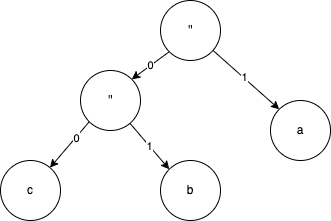
\includegraphics[scale=0.75]{figs/prefixtree.png}
    \caption{Árvore de um código livre de prefixo}
    \label{fig:prefixt}
 \end{figure}
% ----------------------------------------------------------------------------
% Probabilidade -------------------------
\section{Relações fundamentais com a Teoria da Informação}
A codificação é comumente dividida em duas componentes diferentes:\emph{modelo} e \emph{codificador}. 
O \emph{modelo} identifica a distribuição de probabilidade das mensagens baseado em sua semântica e estrutura. 
O \emph{codificador} toma vantagem de um possível \emph{enviesamento (bias)} apontado pela modelagem, e utiliza as probabilidades associadas para reduzir a quantidade de dados necessária para representar a mesma informação (substituindo os símbolos que ocorrem com maior frequência por palavras-código menores).
Isso significa que a codificação está diretamente ligada às probabilidades associadas a cada símbolo do alfabeto de origem.

Nesta seção, vamos construir o embasamento teórico necessário para entender a relação entre as probabilidades associadas e o comprimento das mensagens, e consequentemente criar uma noção dos parâmetros que devem ser maximizados ou minimizados para alcançar uma codificação eficiente.

\subsection{Conceitos básicos em Probabilidade}
Neste texto, iremos trabalhar com espaços de probabilidade finitos,
pois lidamos com alfabetos de origem finitos. Um \textbf{espaço de
  probabilidade finito} é um par $(\Omega, P)$, onde $\Omega$ é um
conjunto finito e $P\colon \Omega \to \mathbb{R}_{\geq 0}$ tal que
$\sum_{\omega \in \Omega} P(\omega) = 1$.

O conjunto $\Omega$ é chamado de \textbf{espaço amostral} e $P$ é
chamada de \textbf{função de probabilidade}. Um \textbf{evento} $E$ é
um sunconjunto de $\Omega$ e sua probabilidade é definida como $P(E)
:= \sum_{\omega \in E} P(\omega)$.

Uma \textbf{variável aleatória} $X$ associa um número real a cada
um dos elementos de $\Omega$. Em outras palavras, $X$ é uma
função que mapeia os elementos do espaço amostral para números
reais. Uma variável aleatória é chamada \textbf{discreta} quando os
valores dos experimentos associados a ela são números finitos ou ao
menos infinitos que podem ser contados.

Podemos descrever melhor uma variável aleatória $X$, atribuindo
probabilidades sobre os valores que esta pode assumir. Esses valores
são atribuídos pela \textbf{distribuição de probabilidade}, denotada
por $p_X$, definida para cada $x\in\mathbb{R}$ como
\begin{equation} \label{eq:dist_prob_def}
p_X(x) = P(\{\omega\in \Omega: X(\omega) = x\}).
\end{equation}
Por simplicidade, de notação utilizamos $P(X=x)$ para denotar
$P(\{\omega\in \Omega: X(\omega) = x\})$. Note que a pré-imagem de $X$
é o espaço amostral e, portanto,
\begin{equation} \label{eq:dist_prob_sum}
\sum_{x ~\in ~im_X}^{}p_X(x) = 1,
\end{equation}
onde $im_X$ denota a imagem de $X$.

O \textbf{valor esperado} (ou \textbf{esperança}) da variável aleatória $X$ é definido como
\begin{equation} \label{eq:exp_val}
\textbf{E}[X] = \sum_{x ~\in ~im_X}^{} xp_X(x).
\end{equation}
%--------------------------------------
% ------------------------------ Entropia
\subsection{Comprimento médio do código}
Seja $p$ a distribuição de probabilidade associada ao alfabeto de
origem $M$. Seja $C: M \to W^+$ um código. Definimos o
\textbf{comprimento/tamanho médio} de $C$ como:
\begin{equation} \label{eq:code_len}
l_a (C) = \sum_{m \in M}^{} p(m) l(C(m)) = \mathbf{E}[l\circ C].
\end{equation}

Estamos interessados em códigos unicamente decodificáveis com o menor
comprimento médio possível. Dada um espaço de probabilidade $(M, P)$ e
um alfabeto código $W$, Um código $C: M \to W^+$ unicamente
decodificável é \textbf{ótimo} se $l_a(C)$ é mínimo, isto é, para
qualquer código unicamente decodificável \emph{C'} temos que
\begin{equation} \label{eq:code_len_optimal}
l_a(C) \leq l_a(C').
\end{equation}
Assim, temos o seguinte problema de otimização
\begin{equation} \label{eq:prog_code_len}
  \begin{array}{rl}
    \min & l_a(C)\\
    \text{sujeito a} &C: M \to W^+ \text{ é um código unicamente decodificável}
  \end{array}
\end{equation}


\subsection{Entropia}
A \textbf{entropia de Shannon} aplica as noções de entropia física
(que representa a aleatoriedade de um sistema) à Teoria da
Informação. Dada uma variável aleatória $X$ com distribuição de
probabilidade $p$, definimos \textbf{entropia} de $X$ como
\begin{equation} \label{eq:entropy}
H(X, p, b) = \sum_{x \in im_X}^{} p(x) \log_b \frac{1}{p(x)},
\end{equation}
onde $b$ é comumente tomado como $2$, mas pode assumir valores inteiros maiores do que~$2$.

Por esta definição temos que quanto menor o enviesamento da função de distribuição de probabilidade relacionada ao sistema, maior a sua entropia. Em outras palavras, a entropia de um sistema está intimamente ligada a sua ``desordem''.

Shannon~\ref{} aplica o mesmo conceito de entropia no contexto da Teoria da Informação, ``substituindo'' o conjunto de estados pelo conjunto de símbolos $M$, isto é, $M$ é interpretado como um conjunto de possíveis símbolos, tendo como $p(m)$ a probabilidade de cada $m \in M$.
Baseado na mesma premissa, Shannon mede a informação de cada símbolo da seguinte forma
\begin{equation} \label{label:info_quantity}
\emph{i(m,b)} = \log_b \frac{1}{p(m)}.
\end{equation}

\subsection{Comprimento de Código e Entropia}
Nas seções anteriores, o comprimento médio de um código  foi definido em função da distribuição de probabilidade associada ao seu alfabeto de origem.
Da mesma forma, as noções de \textbf{entropia} relacionada a um conjunto de mensagens, têm ligação direta com as probabilidades associadas a estas. 
A seguir, será mostrado como podemos relacionar o comprimento médio de um código a sua entropia através da \textbf{Desigualdade de Kraft-McMillan} , e por consequência estabelecer uma relação direta entre \textbf{a entropia de um conjunto de mensagens e a otimalidade do código associada a estas mensagens}.

\begin{theorem}[Desigualdade de Kraft-McMillan]
  \label{thm:kraftmc}
  Sejam $M$ e $W$ conjuntos finitos tais que $|W|\leq 2$. Seja $b :=
  |W|$. Para todo código unicamente decodificável $C: M \to W^+$, vale
  que
  \begin{equation}
    \label{eq:cond_kraft_nec}
    \sum_{m\in M} b^{-l(C(m))} \leq 1.
  \end{equation}
  Além disso, para toda função $f: M\to\mathbb{N}$ tal que
  que satisfaça
  \begin{equation}
    \label{eq:cond_kraft_suf}
    \sum_{m \in M} b^{-f(m)} \leq 1,
  \end{equation}
  existe um código livre de prefixo (e, portanto, unicamente
  decodificável) tal que $l(C(m)) = f(m)$ para todo $m\in M$.
\end{theorem}

Antes de apresentar a demonstração do teorema~\ref{thm:kraftmc}, vamos
explorar as suas consequências para comprimentos de códigos ótimos. 
Uma de suas consequências principais é que o valor da solução
ótima para o problema de otimização~\ref{eq:prog_code_len}
\begin{equation*} 
  \begin{array}{rl}
    \min & l_a(C) = \sum_{m\in M} p(m) l(C(m))\\
    \text{sujeito a} &C: M \to W^+ \text{ é um código unicamente decodificável}
  \end{array}
\end{equation*}
é igual ao valor ótimo do seguinte problema de otimização
\begin{equation*} 
  \begin{array}{rl}
    \min & \sum_{m\in M} p(m) f(m)\\
    \text{sujeito a} &\sum_{m \in M} b^{-f(m)} \leq 1\\
    & f:M\to\mathbb{N}
  \end{array}
\end{equation*}
Além disso, se $f^*$ é uma solução ótima para o problema acima, então
existe um código $C^*: M \to W^+$ livre de prefixo para o qual $f^*$
determina os comprimentos de suas palavras-código. Portanto, podemos
concluir que dentro os códigos unicamente decodificáveis de
comprimento médio ótimo sempre existe um que é livre de prefixo.
 
Vamos ver, em capítulos posteriores, que o algoritmo de Huffman produz
um código livre de prefixo que é ótimo dentre os códigos livres de
prefixo. A discussão acima mostra que tal código também é ótimo dentre
todos os códigos unicamente decodificáveis.

A seguir apresentamos a demonstração da Desigualdade de
Kraft-McMillan.

\begin{proof}[Prova do Teorema~\ref{thm:kraftmc}]
    Primeiramente, mostraremos a equação~\eqref{eq:cond_kraft_nec}.
    
    Seja $C:M\to W^+$ um código unicamente decodificável. Seja $b :=
    |M|$. Seja $l_{\max} = \max_{m\in M} l(C(m))$. Seja $k$ um inteiro
    positivo. Seja
    \begin{equation*}
      W_k := \left\{ C^+(m_1\dotsm m_k):
      m_1,..., m_k \in M\right\}
    \end{equation*}
    e seja
    \begin{equation*}
      W_{k,j} := \left\{
      w \in W_k: l(w) = j
      \right\},
    \end{equation*}
    para $j\in \mathbb{N}$. Temos que
    \begin{align*}
      \left(\sum_{m\in M} b^{-l(C(m))}\right)^k
      &= \prod_{i=1}^k \sum_{m_i \in M} b^{-l(C(m_i))} \\
      &= \sum_{m_1,..., m_k \in M} b^{-\sum_{i=1}^{k} l(C(m_i))} \\
      &= \sum_{w\in W_k} b^{-l(w)}\\
      &= \sum_{j=1}^{k \cdot l_{\max}} |W_{k,j}| \cdot b^{-j}\\
      &\leq \sum_{j=1}^{k \cdot l_{\max}} b^j \cdot b^{-j},
      \quad\text{ pois }|W_{k,j}|\leq b^j\\
      & = k \cdot l_{\max}
    \end{align*}
Logo,
\begin{equation*}
\sum_{m\in M} b^{-l(C(m))} \leq (k \cdot l_{max})^ \frac{1}{k},
\end{equation*}
para todo $k$ inteiro positivo. Como $\lim_{k\to\infty} (k \cdot l_{max})^ \frac{1}{k} = 1$, temos que
\begin{equation*}
\sum_{m\in M} b^{-l(C(m))} \leq 1.
\end{equation*}

Agora vamos provar que a condição~\eqref{eq:cond_kraft_suf} é
suficiente para a existência de um código livre de prefixo com
comprimentos dados por~$f$. Seja $f: M\to\mathbb{N}$
satisfazendo~\eqref{eq:cond_kraft_suf}. Seja $(m_1,\dotsc, m_n)$ tal
que $M = \{m_1,\dotsc, m_n\}$ e $f(m_1) \leq \dotsm \leq f(m_n)$. Seja
$l_i := f(m_i)$ para todo $i\in\{1,\dotsc,n\}$.

Agora vamos construir um código livre de prefixo $C$ em uma ordem
crescente de tamanho, de maneira em que $l(m_i) = l_i$. Seja $l_{\max}$
o maior valor de $l_i$.

\begin{itemize}
  \item Para $j$ de $1$ a $l_{\max}$, defina $W_j$ como todas as
    palavras em $W^+$ de comprimento~$j$ e defina $P_j :=
    \varnothing$.
  \item Para $i$ de 1 a $n$, faça
    \begin{itemize}
    \item seja $C(m_i)$ qualquer palavra em $W_{l_i}\setminus P_{l_i}$,
    \item adicione $C(m_i)$ a $P_{l_i}$ e adicione todas as palavras que
      têm $C(m_i)$ como prefixo a cada $P_{l_j}$ com $j>i$.
    \end{itemize}
\end{itemize}

O procedimento acima produz um código livre de prefixo $C$ desde que
$P_{l_i}$ não seja o conjunto $W_{l_i}$ inteiro para cada
$i\in\{1,\dotsc,n\}$. Ou seja, podemos pensar em $P_{l_i}$ como um
conjunto de palavras proibidas para $m_i$. Seja $b = |W|$. Note que
inicialmente $W_{l_i}$ tem tamanho $b^{l_i}$ e $P_{l_i}$ é vazio, pois
nenhuma palavra é proibida.  Para cada $k<i$, ao atribuir um código de
$W_{l_{k}}$ para $m_k$, adicionamos $b^{l_i - l_k}$ palavras a
$P_{l_i}$.

Suponha para uma contradição que o procedimento falha em atribuir uma
palavra-código para $m_i$. Então
\begin{equation*}
b^{l_i} = |P_{l_i}| = \sum_{k=1}^{i-1} b^{l_i - l_k}.
\end{equation*}
Portanto, dividindo os dois lados por $b^{l_i}$, obtemos
\begin{align*}
  1 = \sum_{k=1}^{i-1} b^{- l_k} <  \sum_{k=1}^{n} b^{- l_k} = \sum_{m\in M} b^{-f(m)}
\end{align*}
o que contradiz o fato que a condição~\eqref{eq:cond_kraft_suf} é satisfeita.
\end{proof}

A seguir vamos ver a relação de entropia com comprimento médio
ótimo. Primeiramente, veremos que a entropia é um limitante inferior
para o comprimento médio de códigos unicamente decodificáveis.

\begin{lemma}[Entropia como limite inferior]
  \label{lem:entropia_inf}
  Dados um conjunto finito $M$ e uma função de probabilidade $p$ para
  $M$, vale que
\begin{equation*}
  H(M, p, b) \leq l_a(C),
\end{equation*}
para todo código unicamente decodificável $C:M\to W^+$ tal que $|W| =
b$.
\end{lemma}

Por outro lado, veremos também que um código de comprimento médio ótimo tem valor no máximo a entropia somada com $1$.

\begin{lemma}[Entropia como limite superior]
  \label{lem:entropia_sup}
  Dados um conjunto finito $M$ e uma função de probabilidade $p$ para
  $M$, existe um código $C:M\to W^+$ livre de prefixo tal que
  \begin{equation*}
    l_a(C) \leq H(M, p, b) + 1
  \end{equation*}
  onde $b = |W|$.
\end{lemma}

  A seguir apresentamos as demonstrações dos lemas acima.
  
  \begin{proof}[Prova do Lema~\ref{lem:entropia_inf}]
    Seja $C:M\to W^+$ um código unicamente decodificável e seja $b :=
    |W|$. Seja $p$ uma função de probabilidade para $M$. Queremos
    provar que $H(M, p,b) - l_a(C) \leq 0$.

    Substituindo $H(M,p, b)$ e $l_a(C)$ por suas definições
    (equação~\eqref{eq:entropy} e equação~\eqref{eq:code_len}, resp),
    temos
    \begin{align*}
      H(M, p, b) - l_a(C)
      &=
      \sum_{m \in M} p(m) \log_b \frac{1}{p(m)}
      - \sum_{m \in M}^{}p(m) l((C(m))) \\
      &=
      \sum_{m \in M} p(m) \left(
      \log_b \frac{1}{p(m)} - l(C(m))
      \right) \\
      &=
      \sum_{m \in M} p(m) \left(
      \log_b \frac{1}{p(m)} - \log_b b^{l((C(m)))}
      \right) \\
      &= \sum_{m \in M}^{}p(m) \log_b \left(\frac{b^{-l(C(m))}}{p(m)}\right)
    \end{align*}

    Pela desigualdade de Jensen, se uma função $f:M\to\mathbb{R}$ é
    côncava, então $\sum_{m\in M} p(m) f(x_m) \leq f(\sum_{m\in M}
    p(m)~x_m)$ para quaisquer $x_m$ positivos. Como a função $\log_b$
    é côncava, podemos aplicar a desigualdade de Jensen ao resultado
    obtido anteriormente para deduzir que
\begin{equation*}
  \sum_{m \in M}^{}p(m) \log_b  \left(\frac{b^{-l(C(m))}}{p(m)}\right)
  \leq
  \log_b\left(\sum_{m \in M} b^{-l(C(m))}\right)
\end{equation*}
Agora, aplicamos a desigualdade de Kraft-McMillan, e concluímos que
\begin{equation*}
  H(M, p, b) - l_a(C)
  \leq
  \log_b 1 = 0,
\end{equation*}
como queríamos demonstrar.
\end{proof}


  \begin{proof}[Prova do Lema~\ref{lem:entropia_sup}]
    Seja $(M,p)$ um espaço de probabilidade finita. Podemos assumir que
    $p(m)>0$ para todo $M$, pois elementos de $M$ com probabilidade
    zero podem ser ignorados.

    Seja $f:M\to\mathbb{N}$ definida como $f(m) = \left \lceil{\log_b
      \frac{1}{p(m)} }\right \rceil$ para todo $m\in M$. Temos que
\begin{align*}
  \sum_{m \in M}^{} b^{-f(m)} &=
  \sum_{m \in M}^{} b^{-\left \lceil{\log_b \frac{1}{p(m)} }\right \rceil} \\
  &\leq \sum_{m \in M}^{} b^{-{\log_b \frac{1}{p(m)} }} \\
  &= \sum_{m \in M}^{} p(m) \\
  &= 1
\end{align*}
Ou seja, $f$ satisfaz a condição~\eqref{eq:cond_kraft_suf}. De acordo
com a desigualdade de Kraft-McMillan existe um código livre de prefixo
$C$ com palavras-código de tamanho dado por $f$, portanto
\begin{align*}
  l_a(C) &=
  \sum_{m \in M} p(m) f(m) \\
  &=  \sum_{m \in M} p(m) \left \lceil{\log_2 \frac{1}{p(m)} }\right \rceil \\
&\leq \sum_{m \in M}^{}p(m) \left(1 + \log_2 \frac{1}{p(m)}\right) \\
&= 1 +  \sum_{m \in M}^{}p(m) \log_2 \frac{1}{p(m)} \\
&= 1 + H(M,p,b).
\end{align*}
\end{proof}


% ------------------- End of chapter 1 -----------------------------




% PARTE
\part{Algoritmos de compressão e pré-processamento}
% ---
\chapter{Algoritmos de compressão sem perda}\label{cap:comp}
% ---

Os algoritmos de compressão podem ser categorizados em duas diferentes classes: os de compressão \textbf{com perda} e \textbf{sem perda}. 
Os \textbf{algoritmos de compressão com perda} admitem uma baixa porcentagem de perda de informações durante a codificação para obter maior performance, muito úteis na transmissão de dados em streaming por exemplo. 
Nos \textbf{algoritmos de compressão sem perda} o processo de codificação deve ser capaz de recuperar os dados em sua totalidade, geralmente utilizados em casos onde não pode haver perda de informações (como por exemplo, compressão de arquivos de texto).

Neste capítulo serão apresentados dois dos principais algoritmos de compressão sem perda (\textbf{Código de Huffman} e \textbf{Lempel-Ziv 77}), bem como algumas variações úteis para o propósito do presente trabalho.

\pagebreak

\section{Código de Huffman} \label{sec:huff}
O \textbf{algoritmo de Huffman} (desenvolvido por David Huffman em 1952 \cite{Huff}) é um dos componentes mais utilizados em algoritmos de compressão sem perda, servindo como base para algoritmos como o Deflate (utilizado amplamente na web).
Os códigos gerados a partir do algoritmos de Huffman são chamados \textbf{Códigos de Huffman}.

O código de Huffman é descrito em termos de como ele gera uma árvore
de código livre de prefixo com alfabeto código $W = \{0,1\}$. A árvore
é binária e assumimos rótulo $0$ nas arestas de um nó para um filho da
esquerda e rótulo $1$ nas arestas de um nó para um filho da direita.
Considere o conjunto de símbolos $M$ e, para cada símbolo $m_i\in M$,
seja $p_i$ a probabilidade associada a $m_i$.

\begin{algorithm}[H]
\caption{Algoritmo de Huffman} \label{alg:huff}
\begin{algorithmic}
	\State $Forest \gets \emph{[]}$\\
	\ForAll{$m_i \in M$} \Comment{Inicializando floresta}
		\State $T \gets newTree()$
		\State $node \gets newNode()$
		\State $node.weight \gets p_i$ \Comment{$w_i = p_i$}
		\State $T.root \gets node$
		\State $Forest.append(T)$ \Comment{Adiciona um nova árvore na floresta}
	\EndFor \\
	
	\While{$Forest.size > 1$}
		\State $T1 \gets ExtractMin(Forest)$ \Comment{Retorna a árvore cuja raiz é mínima, e retira da floresta}
		\State $T2 \gets ExtractMin(Forest)$
		\State $HTree \gets newTree()$
		\State $HTree.root \gets newNode()$ \\
		\State $HTree.root.left \gets T1.root$
		\State $HTree.root.right \gets T2.root$
		\State $HTree.root.weight \gets T1.root.weight + T2.root.weight$
		\State Forest.append(HTree) 
	\EndWhile
\end{algorithmic}
\end{algorithm}

\subsection{Análise assintótica}

Seja $n$ o tamanho do conjunto de símbolos $M$. Para que o algoritmo percorra toda a floresta, formada por uma árvore para cada $m \in M$, serão necessárias $n$ iterações. Considerando que as funções \emph{ExtractMin()} e \emph{.append()} foram construídas a partir de uma fila de prioridades de \textbf{heap} e essas operações podem ser realizadas em tempo $O(\log_2 n)$, o algoritmo será executado em tempo $O(n\log_2 n)$ \cite{Ble}.

\subsection{Corretude}
O teorema a seguir (escrito por Huffman, 1952 \cite{Huff}) afirma
que os códigos de Huffman minimizam o comprimento médio, ou seja, são
ótimos dentre os códigos livres de prefixo.

Nesta seção, considere um alfabeto de origem $M = \{m_1,\dotsc, m_n\}$
com probabilidade $p_i$ para cada símbolo~$m_i$ e alfabeto código $W =
\{0,1\}$. Dizemos que um código $C: M\to W^+$ livre de prefixo é
\textbf{ótimo} se $l_a(C) \leq l_a(C')$ para todo código $C': M\to
W^+$ livre de prefixo.

\begin{theorem}
  \label{thm:otimo_huffman}
  Seja $C_{H}$ um código gerado pelo algoritmo de Huffman. Temos que
  $C_{H}$ é ótimo.
\end{theorem}

Antes de provar o teorema, começamos com uma simples observação.
  
\begin{lemma} \label{lemma:dist_prob_avg_size} Seja $C:M\to W^+$ um código livre de prefixo ótimo. Para todo $i,j \in\{1,\dotsc, n\}$, se $p_i > p_j$, então $l(C(m_i)) \leq l(C(m_j))$
\end{lemma}
  \begin{proof}
    Sejam $i,j \in\{1,\dotsc, n\}$ e suponha que $p_i > p_j$.  Seja
    $w_i = C(m_i)$ e seja $w_j = C(m_j)$. Para efeito de contradição,
    assuma que $l(w_i) > l(w_j)$.  Agora construa um novo código $C'$,
    trocando $w_i$ por $w_j$. Ou seja, $C'(m_k) = C(m_k)$ para todo $k
    \in \{1,\dotsc, n\} \setminus \{i,j\}$, $C'(m_i) = w_j$ e $C'(m_j)
    = w_i$.  Dado o comprimento médio $l_a(C')$ é
 \begin{align*}
   l_a(C') &= l_a(C) + p_j\cdot(l(w_i) - l(w_j)) + p_i\cdot(l(w_j) - l(w_i)) \\
   &= l_a(C) + (p_j - p_i)(l(w_i) - l(w_j))\\
   &< l_a(C),
 \end{align*}
 pois $p_j - p_i < 0$ e $l(w_i) - l(w_j)>0$. Isso contradiz o fato do
 código $C$ ser ótimo.
  \end{proof}

\noindent \textbf{Nota:} Perceba que em uma árvore de Huffman, o comprimento de uma palavra-código também representa seu nível na árvore.

\begin{proof}[Prova do Teorema~\ref{thm:otimo_huffman} (Blelloch, 2013 \cite{Ble})]
A prova se dará por indução sobre o tamanho $n$ de $M$. Para a base,
tome $n=2$. Nesse caso, o resultado é trivialmente verdadeiro
considerando que o algoritmo de Hufman gera um código que atribui um
bit pra cada símbolo de~$M$. Assuma então que $n>2$ para o passo
indutivo. Sejam $x$ e $y$ nós associados a símbolos $m_a$ e $m_b$
respectivamente tais que $p_a \leq p_b \leq p_i$ para todo $i \in
\{1,\dotsc,n\}\setminus\{a,b\}$. Ou seja, $x$ e $y$ poderiam ser os nós escolhidos como o primeiro par pelo algoritmo de Huffman.

Seja $m'$ um novo símbolo com probabilidade $p_a+p_b$ e seja $M' =
(M\cup\{m'\})\setminus\{m_a, m_b\}$. Note que $|M'| < n$. Seja $T'$
uma árvore obtida pelo algoritmo de Huffman para $M'$. Por hipótese de
indução o código $C'$ da árvore $T'$ é ótimo para $M'$. A árvore $T$
obtida pelo algoritmo de Huffman é a árvore $T'$ adicionando os nós
$x$ e $y$ como filhos do nó associado a $m'$. Seja $C$ o código da
árvore $T$.

Agora iremos comparar com um código ótimo. Afirmamos que
\begin{equation}
 \label{irmaos}
\text{Existe um código $C^*$ livre de prefixo ótimo com árvore $T^*$
  tal que $x$ e $y$ são \textbf{irmãos}.}
\end{equation}
Seja $z$ o pai de $x$ e de $y$ em $T^*$. Note que a árvore obtida a
partir $T^*$ pela remoção de $x$ e $y$ e associando $z$ ao símbolo
$m'$ (de probabilidade $p_a+p_b$) gera um código $C^{**}$ para $M'$. Pela
otimalidade de $C'$, temos que
\begin{equation*}
  l_a(C^*)
  =
   l_a(C^{**})+p_a+p_b
  \geq
  l_a(C')+p_a+p_b
  =
  l_a(C),
\end{equation*}
o que mostra a otimalidade de $C$.


Finalmente provamos a afirmação em~\eqref{irmaos}.  Dado um código
$C''$ livre de prefixo ótimo com árvore $T''$, pelo
lema~\ref{lemma:dist_prob_avg_size}, sabemos que os símbolos com as
menores probabilidades estão nos menores níveis de $T''$ (ou seja,
associados a palavras-código de maior comprimento). Portanto, $x$ e
$y$ são folhas em $T''$. Seja $w \in\{x,y\}$ tal que $w$ é $x$ se o
nível de $x$ é menor ou igual ao nível de $y$ e seja $v$ o nó em
$\{x,y\}\setminus\{w\}$. (Note que $w$ só pode ser $y$ no caso em que
$p_a = p_b$, pelo lema~\ref{lemma:dist_prob_avg_size}). Seja $z$ o pai
de $w$. Se $w$ é o único filho de $z$, então poderíamos mudar $w$ para
$z$ (pois $z$ não é associado a nenhum símbolo dado que $C''$ é livre
de prefixo). Portanto, $w$ tem um nó \textbf{irmão} $w'$. Se $w'$ não
é $v$, trocar $w'$ com $v$ gera um código de comprimento menor ou
igual ao de $C''$ pelo lema~\ref{lemma:dist_prob_avg_size}. 
\end{proof}


\section{Lempel-Ziv 77 (LZ77)}

\subsection{Algoritmos de Lempel-Ziv}
Nos anos de 1977 e 1978, Jacob Ziv e Abraham Lempel publicaram dois artigos apresentando os algoritmos \textbf{LZ77} e \textbf{LZ78} \cite{LZ}, que serviriam como base para uma família de algoritmos de compressão (conforme mostrado na Figura~\ref{fig:lz77}), chamados de algoritmos de \textbf{Lempel-Ziv}.
Os algoritmos de Lempel-Ziv realizam o processo de compressão baseado em um \textbf{dicionário} de mensagens vistas anteriormente (diferente do \nameref{alg:huff}, que utiliza a probabilidade associada a cada símbolo). 
Tanto o LZ77 quanto o LZ78 têm um funcionamento parecido, que se resume em substituir partes da entrada por referências a partes iguais anteriormente processadas, e diferem na maneira em que procuram por repetições a serem substituídas. 

\begin{figure}[h]
   \centering
   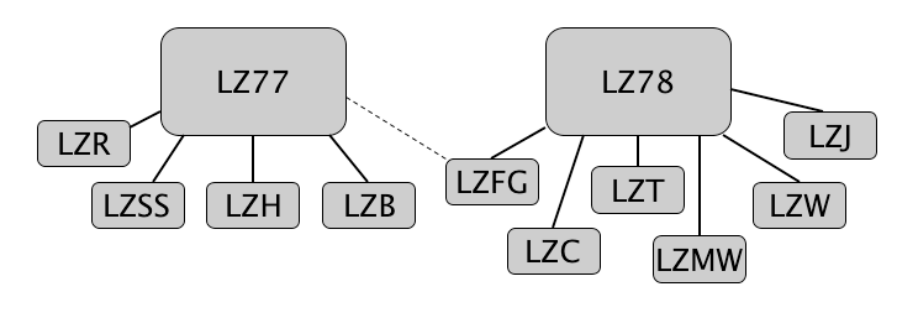
\includegraphics[scale=0.75]{figs/lz77fam.png}
    \caption{Familia de algoritmos Lempel Ziv}
    \label{fig:lz77}
 \end{figure}

\subsection{Descrição do LZ77}
O LZ77 e suas variações utilizam a técnica de \emph{janela deslizante} para encontrar mensagens correspondentes. 
A janela é dividida em duas partes separadas por um \emph{cursor} (que se move conforme novas mensagens são codificadas).

A mensagem à esquerda do cursor é chamada de \textbf{dicionário}, e contém todos os símbolos já codificados. Já a mensagem à direita do \emph{cursor} é chamada de \textbf{lookahead buffer}.
A ideia geral do algoritmo é substituir as mensagens do \emph{lookahead buffer} por \textbf{tokens}, onde cada \emph{token} é constituído por uma \emph{tupla} que ``aponta''  para a maior mensagem correspondente a cadeia no início do \emph{lookahead buffer}.

A \emph{tupla} que constitui os \emph{tokens} é formada por três valores:
um valor inteiro que indica quantas posições para trás o \emph{cursor} deve retornar até encontrar o início da cadeia, 
um segundo valor inteiro indicando o tamanho da cadeia,
e um caracter (preenchido com $m_{cursor}$ ou $null$ para \textbf{tokens não vazios}).

Os \emph{tokens} podem ser vazios, quando não encontramos nenhuma mensagem correspondente, neste caso, os dois primeiros valores da \emph{tupla} são preenchidos com zeros.
Por exemplo, se durante a compressão de um texto encontrássemos o símbolo ``a'' pela primeira vez (isso é, não existe correspondência pra ele no \emph{dicionário}), a saída seria o \emph{token vazio} $(0, 0, $``a''$)$.

\begin{algorithm}[H]
\caption{Algoritmo Lempel-Ziv 77} \label{alg:lz77}
\begin{algorithmic}

	\State $cursor \gets 0$
	\State $tokens \gets []$

	\While{$cursor < M.size()$}
		\State $position, len \gets findLongestMatch(M, cursor)$ \Comment{Retorna a posição e tamanho da maior cadeia correspondente}
		\If{$len > 0$} \Comment{Cria novo token, que aponta para a cadeia encontrada}
			\State $tokens.append([position, len, null])$
			\State $cursor \gets cursor + len$
		\Else
			\State $tokens.append((0, 0, M[cursor]))$ \Comment{Token vazio}
			\State $cursor \gets cursor + 1$
		\EndIf
	\EndWhile
\end{algorithmic}
\end{algorithm}

\subsection{Função ``\emph{findLongestMatch}'' }
O \emph{LZ77} possui um processo de decodificação muito eficiente, porém consome muitos recursos computacionais na codificação. 
Isto é, ele é mais eficiente para casos onde pretende-se decodificar o arquivo múltiplas vezes, ou ainda decodificá-lo numa máquina com menor poder computacional. 
O ``gargalo'' da compressão está na técnica de busca pelo \emph{dicionário} para encontrar a mensagem correspondentes mais longa.

O método convencional utilizado é a \textbf{busca linear}, que consiste em comparar cada posição no dicionário com o \emph{lookahead buffer} e selecionar a maior correspondência encontrada. 
Tome $N$ como o tamanho do dicionário e $M$ como o tamanho do \emph{lookahead buffer}, no pior caso, a busca linear é realizada em tempo $O(NM)$. 
A busca será executada $M + N$ vezes, isto é, a complexidade geral do algoritmo é $O( N^{2}M + M^{2}N)$.

\subsection{Melhorias na performance da função ``\emph{findLongestMatch}'' }

Uma das possíveis abordagens para melhorar a busca linear é utilizar estruturas de dados auxiliares, que indexam os símbolos do dicionário para tornar a busca mais rápida.
Bell (1993) \cite{TD}  testa diferentes estruturas de dados (árvores trie, hash tables, árvores binárias de busca entre outros). 
Para este trabalho utilizaremos a \textbf{lista ligada} como estrutura de dados auxiliar (principalmente por possuir uma implementação mais simples). 

Para construir uma estrutura de dados auxiliar com lista ligada, podemos criar uma lista para cada símbolo no dicionário, que contenha os índices onde o símbolo pode ser encontrado.  
Para limitar a janela de busca, podemos construir a lista como uma \emph{fila}, onde ao atingirmos a capacidade máxima da janela de busca, removemos o menor índice (que estaria no início da fila). 
Note que, o tamanho máximo da lista depende da quantidade de bits que queremos utilizar para construir o \emph{token}.

Encontramos a maior mensagem correspondente, comparando o \emph{lookahead buffer} com as cadeias de símbolos iniciadas a partir de índices contidos na lista que corresponde ao primeiro símbolo do \emph{lookahead buffer}.
Neste contexto, o pior caso ocorrerá quando todos os símbolos no dicionário forem iguais, pois todas as posições no dicionário seriam checadas (levando a uma performance equivalente a da busca linear).
Entretanto, para uma base de dados de texto real com grande quantidade de dados isso raramente acontece, e apenas uma quantidade $K \ll N$ de possíveis mensagens são realmente checadas.

\section{Compressão baseada em palavras}
A implementação padrão para a maioria dos algoritmos de compressão utiliza como \emph{alfabeto de origem} elementos de 8 bits (também conhecidos como \textbf{\emph{caracteres}}).
Tal método limita a correlação de cadeias mais longas, e tem sua eficiência limitada quando aplicado a grande quantidade de dados. 
Em contrapartida, se definirmos cada símbolo do \emph{alfabeto de origem} como uma sequência caracteres, poderíamos tirar vantagem de longas correspondências e talvez obter melhores resultados na compressão.

Quando a natureza dos dados é previamente conhecida, podemos tomar vantagem da sua estrutura para definir os símbolos de uma maneira mais eficiente. 
Em especial, linguagens ``faladas'' possuem uma estrutura hierárquica bem definida, que vai desde o agrupamento de letras em sílabas, silabas em palavras, palavras em frases e assim por diante. 

Neste contexto, definiremos uma \textbf{\emph{palavra}} como uma sequência maximal de \emph{caracteres} alfanuméricos, divididos por sequências de caracteres não alfanuméricos chamados \emph{separadores} (baseado na definição feita por Bentley (1986) \cite{Bentley}).
A compressão baseada em palavras é uma modificação dos algoritmos de compressão clássicos, que considera cada palavra como um símbolo (i.e, o \emph{alfabeto de origem} passa a ser composto por \emph{palavras}, não por \emph{caracteres}).

\subsection{Huffword} \label{sub:huffw}
O método de compressão \emph{Huffword} é uma modificação da implementação canônica do \emph{código de Huffman}. 
Desenvolvido por Moffat e Zobel (1994) \cite{Moffat}, ele utiliza \emph{palavras} em seu alfabeto de origem.

O algoritmo funciona de maneira bem similar à implementação canônica, o arquivo é pré-processado separando as \emph{palavras} e os \emph{separadores} como duas entradas distintas.
Depois o algoritmo de Huffman canônico é aplicado a cada uma das partes, sendo que as probabilidades agora estão associadas às palavras e não mais aos caracteres. 
A codificação associada a entrada também é armazenada em duas \emph{strings} distintas, assim como as tabelas de códigos também são distintas.
 
 \subsection{WLZ77}
Platos (2008) \cite{Platos} implementa a versão do LZ77 baseado em palavras (também chamado WLZ77) aplicando uma ideia semelhante à apresentada anteriormente . 
 O arquivo é pré-processado para obter uma lista de \emph{palavras} e \emph{separadores}. 
 Ao contrário do ~\nameref{sub:huffw} as palavras e separadores são processados simultaneamente pela implementação canônica do LZ77, gerando uma sequência única de \emph{tokens}.
 
 Vale notar que, neste caso, o último elemento da \emph{tupla} no token não é mais um caractere e sim uma palavra. Isso significa que para o caso dos \emph{tokens vazios}, o tamanho do \emph{token} irá variar de acordo com o tamanho da palavra.
 
 % ---
 \chapter{Clusterização de dados aplicada a textos}\label{cap:clus}
 % ---
 
 O processo de clusterização de dados consiste em agrupar os objetos (que compõe o conjunto de dados) em $n$ diferentes \textbf{agrupamentos} (clusters), de maneira em que os objetos de um mesmo grupo sejam similares e os de grupos diferentes dissimilares.
 Para isto, faz-se essencial uma definição clara da similaridade entre os objetos, que pode variar dependendo da natureza do dado em análise.
 
 Podemos construir o processo de clusterização de diferentes maneiras \cite{Goog2}: Na \textbf{clusterização sem sobreposição} cada objeto deve pertencer a exatamente um cluster. 
 Em contrapartida podemos agrupar os objetos permitindo algumas sobreposições. 
 Podemos ainda clusterizar dados por \textbf{hierarquia}, onde os dados são organizados em níveis (quase como uma árvore).
 
 \begin{figure}[H]
   \centering
   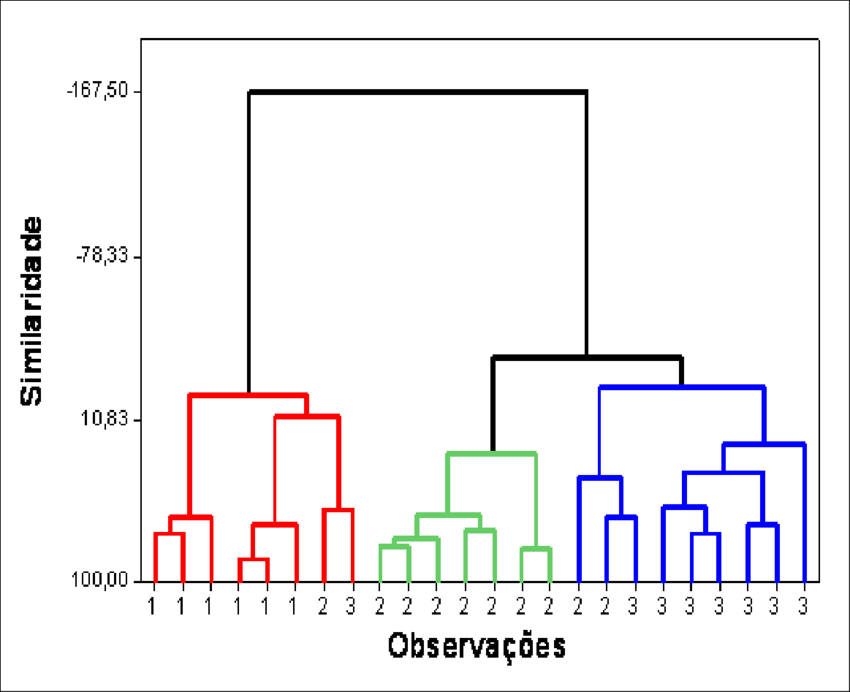
\includegraphics[scale=0.50]{figs/cluster_h.png}
    \caption{Exemplo de agrupamento hierárquico}
    \label{fig:clusterh}
 \end{figure}
 
 \pagebreak
 
 \section{Similaridade em dados textuais}
 Conforme introduzido anteriormente, definir uma métrica de similaridade entre os objetos é essencial para o funcionamento dos algoritmos de clusterização.
 Para o propósito deste trabalho, iremos explorar técnicas que extraem essa similaridade em dados textuais.
 
 Para uma base de dados textual,  utilizaremos o termo \textbf{``texto bruto''}  para se referir ao conteúdo de cada registro na base de dados. 
 Também adotaremos o termo \textbf{documento} para partições dos dados (por exemplo, uma linha da tabela).
 Estenderemos a definição de \emph{palavras} e \emph{separadores} utilizadas no capítulo anterior, definidas sob um ponto de vista linguístico (não relacionados diretamente a notação de conjuntos definida no capítulo ~\ref{chapter:fund}).
 
 \subsection{Vetorização TF-IDF}
Análise de texto é umas das aplicações mais exploradas no campo dos sistemas inteligentes.
Porém, pode ser uma tarefa difícil utilizar texto bruto como entrada para os algoritmos de \emph{machine learning}. 
Geralmente, tais algoritmos ``lidam melhor'' com características numéricas.
 
O processo de transformar documentos em vetores de características numéricas é conhecido como \textbf{vetorização} \cite{Qaiser}. 
Em geral, procuramos uma medida que atribua pesos a cada palavra, de acordo com a sua ``importância'' no documento.

Poderíamos atribuir pesos às palavras de maneira direta e intuitiva, atrelando o peso diretamente a frequência em que aquela palavra ocorre em um documento.
Chamamos esta medida de \textbf{TF} (\emph{term frequency}).

\begin{equation}\label{eq:tf}
tf(t, d) = \frac{count(t \in d)}{count(d)}
\end{equation}

Onde $t$ é a palavra (ou termo) alvo da medição, e $d$ é o documento que contém a palavra $t$  e pertence a coleção de documentos $D$.

Entretanto, algumas palavras (como ``and'' ou ``him'' no inglês) adicionam pouca ou nenhuma informação relevante para o texto em si, apesar de sua alta frequência, essas palavras são conhecidas como \textbf{\emph{stop words}}.
Remover as \emph{stop words} pode diminuir ruídos nos dados utilizados para o modelo de classificação, sendo um recurso muito importante para a construção de clusters com maior significado semântico.

Para compensar este fator, o \textbf{IDF} (\emph{inverse document frequency}) pondera o quão ``incomum'' é um determinado termo entre diferentes documentos, atribuindo valores baixos a termos que se repetem muito em diferentes documentos \cite{Qaiser}.

\begin{equation}\label{eq:idf}
idf(t, D) = \log \frac{len(D)}{count(d \in D : t \in d)}
\end{equation}


A métrica \textbf{TF-IDF} multiplica as equações~\ref{eq:idf} e ~\ref{eq:tf}, de maneira que a informação da frequência de um termo é ponderada pela sua ``exclusividade'' entre os documentos.
Obtemos assim uma métrica que aproxima a zero os símbolos menos relevantes, e atribuí valores maiores a símbolos ``mais relevantes''.

\begin{equation}
tfidf(t, d, D) = tf(t, d) \times idf(t, D)
\end{equation}

 \section{Redução de Dimensionalidade}
 Em casos em que a base de dados possuem uma quantidade elevadas de dimensões, 
reduzir a dimensionalidade significa procurar variáveis que possuem dependência entre si.
No geral, busca-se manter apenas características relevantes aos dados, reduzindo sua complexidade e o poder computacional necessário para processar estes dados.

 \subsection{PCA}
 O PCA (ou \emph{principal component analysis}) é formado por um procedimento algébrico, 
 que reduz as variáveis correlacionadas em um conjunto de variáveis não relacionadas (linearmente) chamadas \emph{principal components} (PCs), iterativamente \cite{Jolliffe}.
 No contexto da clusterização, o PCA é utilizado principalmente para transformar dados com muitas dimensões em uma representação com menores dimensões (usualmente duas dimensões, facilitando a análise gráfica dos dados).
 
 
 \section{Clusterização K-means}
O método de clusterização \emph{k-means} (ou algoritmo de Lloyd's \cite{Lloyd}) é um algoritmo iterativo que particiona os dados em $k$ clusters, definidos por \textbf{pontos centrais} (onde $k$ é uma das entradas para o algoritmo).
A ideia em geral é encontrar os melhores $k$ pontos centrais, isto é, posicionar estes pontos de maneira a minimizar a distância dos dados aos pontos centrais mais próximos. 
Podemos definir o k-means da seguinte forma:
 \begin{enumerate}
 	\item Escolha os $k$ primeiros pontos centrais. A escolha pode ser \textbf{aleatória}, ou utilizando o \emph{k-means++} (algoritmo para inicializar os pontos centrais).
	\item Calcule a distância de cada dado em relação a cada ponto central.
	\item Atribua cada dado ao ponto central mais próximo.
	\item Calcule a distância média entre os pontos e seus respectivos centros para cada cluster, e obtenha novas localizações para os pontos centrais (de maneira a minimizar a distância média).
	\item Repita os passos 2, 3, e 4 até que os clusters não mudem, ou atingir o número máximo de iterações.
\end{enumerate}
 
 \begin{figure}[H]
   \centering
   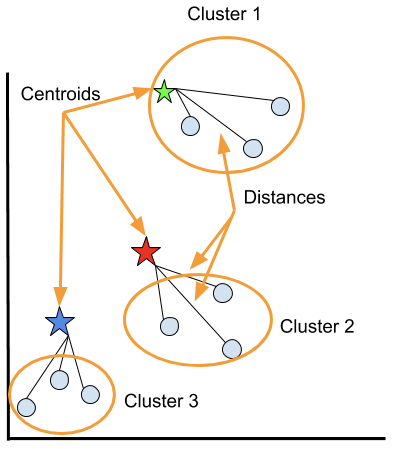
\includegraphics[scale=0.40]{figs/kmeans.png}
    \caption{Exemplo de clusterzacao k-means}
    \label{fig:kmeans}
 \end{figure}
 
 
 \subsection{Método de elbow}\label{ssec:elbow}
 O resultado do \emph{k-means} é diretamente afetado pelo número de clusters definidos na inicialização do algoritmo.
 Existem diversas formas para determinar o número ``ideal'' de clusters, uma delas é o \textbf{método de elbow} \cite{Humaira}.
 
 Neste método, executa-se o \emph{k-means} para um range pré-definido de valores em $k$. 
 Depois disso, calcula-se a soma das distâncias quadráticas (também chamada de \textbf{inércia}) de cada ponto para o seu respectivo ponto central.
 0 resultado para cada $k$ é plotado em um gráfico de linha (conforme mostra a figura~\ref{fig:elbow}).
 Seleciona-se o número de clusters que corresponde ao ``cotovelo'' (elbow) do gráfico.
 
\begin{figure}[H]
   \centering
   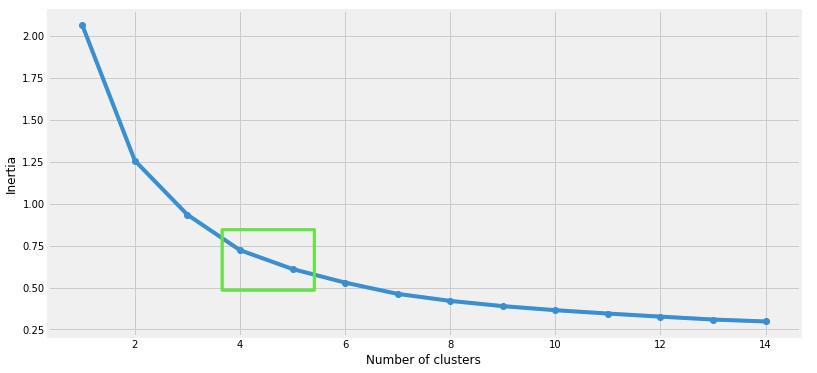
\includegraphics[scale=0.40]{figs/elbowex.png}
    \caption{Método de elbow}
    \label{fig:elbow}
\end{figure}

 
 





% PARTE
\part{Aplicação: Melhoria na compressão de dados textuais em larga escala através da Clusterização}
\chapter{Clusterização como pré-processamento na compressão de textos}
Nos capítulos anteriores, construímos a estrutura teórica necessária para compreender a \emph{compressão de texto} e sua relação com a \emph{teoria da informação}.
Fica claro que os algoritmos apresentados, tomam vantagem de alguma redundância presente na mensagem para representar a informação de maneira mais eficiente.
Isto é, a \textbf{eficiência} destes algoritmos está intimamente ligada com a \textbf{entropia} do texto a ser comprimido,
 nos dando um indício de que \textbf{minimizar} a entropia, pode ser uma forma de \textbf{maximizar} a \textbf{taxa de compressão}.
 
O capítulo~\ref{cap:clus} apresenta uma técnica para organizar o texto em \emph{grupos de mensagens similares} (\textbf{clusterização}), o que significa diminuir a variação de termos dentro de cada cluster (ou reduzir a sua \textbf{entropia}).
Neste capítulo, exploraremos de maneira empírica a relação entre a entropia associada a um texto e a taxa de compressão dos algoritmos apresentados no capítulo~\ref{cap:comp}.

A seguir, será descrito um experimento que utiliza a \textbf{clusterização} como pré-processamento de uma base de dados textual, visando uma melhora na performance dos algoritmos de compressão \emph{sem perda}.
Foram realizados experimentos utilizando ou não o pré-processamento, afim de medir o impacto da clusterização para os algoritmos testados (que serão listados em seções posteriores).

Todo o experimento foi desenvolvido em \emph{Python} (principalmente ao seu vasto ferramental para manipulação de dados) e o código está disponível no GitHub [TODO REF GITHUB].
O código fonte está organizado nas seguintes camadas:
\begin{itemize}
	\item \textbf{dataset}: Contém os arquivos \emph{.csv} que serão carregados como base de dados.
	\item \textbf{compressors}: Classes e scripts com a implementação dos codificadores utilizados.
	\item \textbf{stackexchange\_compression\_experiments.ipynb}: \emph{Python notebook} com o código fonte de todo o experimento (pré-processamento dos dados, particionamento das bases, aplicação dos algoritmos de compressão, plot de gráficos, entre outros).
\end{itemize}
\pagebreak

\section{Escolha e tratamento de dados}
Para a realização do experimento, a escolha da base de dados é uma etapa primordial.
É necessária uma base de dados robusta, com uma grande quantidade de \textbf{texto} e que permita a criação de \emph{clusters} contendo assuntos diversos.

Para o experimento, foi selecionada a base de dados ``\emph{Transfer Learning o Stack Exchange Tags}'', que está disponível no \emph{kaggle}.
Trata-se de um conjunto de dados extraídos do website \emph{Stack Exchange} (um grande forum online, com conteúdo de diversos assuntos e uma grande variedade de dados textuais).

As principais informações contidas na base de dados são o título das questões, o conteúdo da questões (em formato HTML) e as \emph{tags} que classificam o conteúdo em diferentes tópicos (biologia, culinária, criptografia, robótica e viagem).
O tamanho total da base de dados original é de aproximadamente \textbf{50MB}. 

\subsection{Criação do dataframe principal}
Os dados extraídos do \emph{kaggle} estavam originalmente separados em arquivos \emph{csv}, um para cada tópico.
Os arquivos foram concatenados e somados em um único \emph{dataframe}, utilizando a biblioteca $pandas$.
Para cada arquivo, foram selecionadas \textbf{1500} linhas (devido as limitações do hardware utilizado para o teste), o \emph{dataframe} final gerado possuí aproximadamente \textbf{7MB} de informação.


\begin{lstlisting}[language=Python, caption=Carregando base de dados]
# Loading dataframe
def load_dataset(dataset_name):
    f_path = 'dataset/stack-exchange-tags/{dataset}.csv'.format(dataset = dataset_name)
    full_path = os.path.join(os.getcwd(), f_path)
    return p.read_csv(full_path, index_col=0, nrows=1500)

ds_names = ['biology', 'cooking', 'crypto', 'diy', 'robotics', 'travel']
frames = [load_dataset(name) for name in ds_names]
df = p.concat(frames)
\end{lstlisting}

\subsection{Sanitização das colunas}
Como parte da preparação dos dados para o experimento, as colunas do \emph{dataframe} foram \textbf{sanitizadas}.
O processo de sanitização consiste em remover as \emph{stopwords}, pontuações, tags \emph{html} e outras informações que podem ser problemáticas para o experimento (principalmente na etapa de clusterização).
A partir da sanitização, novas colunas foram geradas no \emph{dataframe} (contendo o pré-fixo ``sanitized').

\begin{lstlisting}[language=Python, caption=Sanitização do texto]
from wordcloud import STOPWORDS
import re\
stop_words = set(STOPWORDS)

# # Sanitizing columns
def sanitize_column(data):
    # convert to lower
    data = data.lower()
    # strip html
    data = re.sub(r'\<[^<>]*\>','',data.lower())
    #removing pontuation
    data = re.sub(r'[^a-zA-Z0-9]',' ',data)
    # Remove new lines and tabs
    data = re.sub(r'\s',' ',data)

    #strip data
    data = data.strip()

    #Spling words
    data = data.split()
    
    #Remove extra blank space
    data = list(filter(lambda s: s != ' ', data))

    # Remove stop words
    data =  list(filter(lambda s: s not in stop_words,data))

    #remove single chars words
    data = list(filter(lambda s: len(s) > 1, data))

    return data
def array_column_to_text(column):
    text = ''
    for w in column:
        for s in w:
            text += ' ' + s 
    return text
df['sanitezed_content'] = df['content'].apply(sanitize_column)
\end{lstlisting}

A biblioteca \textbf{worldcloud} foi utilizada para visualizar a distribuição dos termos de maneira gráfica.
A Imagem~\ref{fig:wordcloud1} demonstra a representação gráfica das palavras de acordo com a sua frequência.

 \begin{figure}[H]
   \centering
   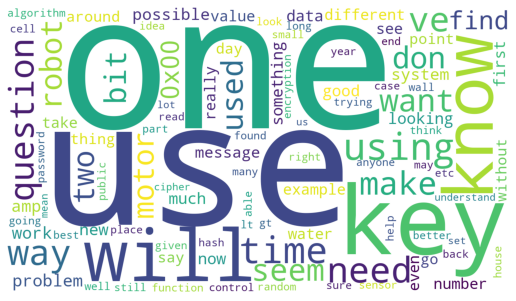
\includegraphics[scale=0.50]{figs/wordcloud1.png}
    \caption{Cluster de palavras}
    \label{fig:wordcloud1}
 \end{figure}

\section{Compressão de textos}
Os testes foram realizados com dois algoritmos clássicos de compressão \emph{sem perda} e suas versões baseadas em palavras (\textbf{Huffman}, \textbf{Huffword}, \textbf{LZ77}, \textbf{WLZ77}).
Neste conjunto de algoritmos estão presente algoritmos baseados em \emph{probabilidades associadas} e \emph{dicionários}
Os testes foram realizados sobre quatro algoritmos de compressão \textbf{sem perda} (apresentados no capítulo~\ref{cap:comp}), sendo dois baseados em \emph{caracteres} e os outros dois em \emph{palavras}
Uma hipótese razoável a ser validada é que com a versão baseado em palavras, o impacto da clusterização na taxa de compressão seja mais significativo.
A seguir, serão descritos alguns detalhes específicos da implementação dos compressores para o experimento (dando ênfase nos detalhes não contidos nos algoritmos em pseudo-código apresentados no capítulo~\ref{cap:comp}).

\subsection{Classes auxiliares}
Para facilitar a reutilização de código na aplicação dos diferentes compressores, foi criada a classe auxiliar (\emph{TextCompressor}).
Nesta classe, são expostos os método \emph{encode(text)} e \emph{decode()} que servem como um ``contrato'' para a implementação dos algoritmos de compressão.
Cada classe que modela um compressor herda da classe base \emph{TextCompressor}, criando sua própria implementação dos métodos \emph{encode} e \emph{decode}.


\begin{lstlisting}[language=Python, caption=Classe TextCompressor]
class TextCompressor:
    def __init__(self):
        self.originaltext = None
        self.stats = None
    def encode(self, text):
        self.originaltext = text
        pass
    def decode(self):
        pass
\end{lstlisting}

Outra classe auxiliar implementada foi a \emph{CompressionStats}, uma interface para padronizar a leitura das métricas.

\begin{lstlisting}[language=Python, caption=Implementaçào da classe base CompressionStats]
class CompressionStats:
    def _avg_code(self):
        return (self.compressedtextsize / self.originaltextsize) * 8
    def _compression_rate(self):
        return 100 - (self.compressedtextsize / self.originaltextsize) * 100
    def __init__(self, originaltext, compressedtext):
        self.originaltextsize = len(originaltext)
        self.compressedtextsize = len(compressedtext)
    def __str__(self) -> str:
        return stats_text.format(csize=self._avg_code(), osize=self.originaltextsize, nsize=self.compressedtextsize, crate=self._compression_rate())
\end{lstlisting}

\subsection{Compressão baseada em palavras}
Para a implementação dos algoritmos baseados em \textbf{palavras}, boa parte do código fonte utilizado nos algoritmos ``canônicos'' foram reutilizados.
Como o \emph{Python} é uma linguagem de \textbf{tipagem dinâmica}, a implementação ``canônica'' interpreta a entrada como um vetor de \emph{símbolos} (sem necessariamente distinguir o tipo de símbolo).
Com isso, podemos reaproveitar grande parte das funções escritas independente do alfabeto de origem utilizado. 

O \emph{Huffword} computa as \emph{palavras} e \emph{separadores} como duas entradas distintas.
Para dividir a entrada entre \emph{palavras} e \emph{separadores}, foi utilizada a biblioteca \emph{re}, que permite executar buscas em \emph{strings} utilizando \emph{regex}.
A mesma lógica é aplicada ao \emph{WLZ77}, diferindo do fato que desta vez, as \emph{palavras} e \emph{separadores} são processadas em um único vetor.

\begin{lstlisting}[language=Python, caption=Função \emph{encode} para o \emph{Huffword}]
def _build_huffword_code(seq):
    freqs = frequency_dictionary(seq)
    huff_tree = canonical.build_huff_tree(freqs)
    code_table= canonical.build_code_table(huff_tree)
    return code_table
    
def huffword_encode(text):
    # Words huff tree
    words = re.findall(r'\w+', text)
    words_code = _build_huffword_code(words)

    # Non words huff tree
    nonwords = re.findall(r'\W+', text)
    nonwords_code = _build_huffword_code(nonwords)

    encoded_string = ""

    # When text start with non-word append 0, otherwise append 1
    starts_with = 0
    if text.startswith(words[0]):
        starts_with += 1
    
    # Append starts with as the first char
    encoded_string += str(starts_with)

    # Encode intercalating words and nonwords
    w_index = 0
    nw_index = 0

    #When starts with non words
    if not starts_with:
        encoded_string += nonwords_code[nonwords[0]]
    
    while w_index < len(words) or nw_index < len(nonwords):
        if w_index < len(words):
            word = words[w_index]
            encoded_string += words_code[word]
            w_index += 1
        
        if nw_index < len(nonwords):
            nonword = nonwords[nw_index]
            encoded_string += nonwords_code[nonword]
            nw_index += 1
    
    return {'encoded' : encoded_string,
            'words_meta' : (words, words_code),
            'non_words_meta': (nonwords, nonwords_code)}
\end{lstlisting}



\section{Partição de dados}
Os testes com os algoritmos de compressão foram realizados com duas estratégias diferentes de partição.
Na primeira, os dados são particionados \textbf{aleatoriamente} em $n$ partes.
Já para o teste com a clusterização, os mesmos dados são particionados em $n$ \emph{clusters} criados pelo algoritmo \emph{k-means}.
Em ambos os casos, cada algoritmo de compressão foi executado sobre as $n$ partições (grupos) e as métricas foram computadas por média média aritmética simples.

\subsection{Partição aleatória} \label{ssec:randomp}
Para o teste com partição aleatória, o \emph{dataframe} original foi dividido em $n$ partes iguais.
É importante que tais divisões sejam aleatórias, afim de evitar possíveis ruídos no teste.

Para garantir a aleatoriedade, foi utilizado o método $.sample()$ da biblioteca $pandas$. 
Este método cria uma amostra aleatória de items para um determinado eixo do objeto. 
O parâmetro $frac=1$ faz com que o método retorne uma amostra com todos os dados originais (porém de maneira randômica).
Em seguida, o vetor foi fracionado pela função $array\_split()$ da biblioteca $numpy$.

\begin{lstlisting}[language=Python, caption=Partição aleatória de dados]
# Data to compress: Compress the original data raw
raw_text = df['content']

#Shuffle raw text
shuffle = raw_text.sample(frac=1)
partitions = np.array_split(shuffle, n_partitions)
\end{lstlisting}

\subsection{Clusterização}
Para o teste com partição por clusterização, o algoritmo \emph{k-means} foi utilizado.
A clusterização se inicia transformando os dados textuais em \textbf{vetores de características}, utilizando a técnica de vetorização \emph{TF-IDF}. 
O vetor de características passa por uma redução de dimensionalidade via \emph{PCA} (reduzindo os dados em \textbf{duas} componentes principais, para melhor visualização).

\begin{lstlisting}[language=Python, caption=Vetorização dos dados]
def identity_tokenizer(text):
  return text

vect = TfidfVectorizer(tokenizer=identity_tokenizer,lowercase=False)
tf_idf = vect.fit_transform(df['sanitezed_content'].values)
tf_idf_norm = normalize(tf_idf) # To PCA running
tf_idf_arr = tf_idf_norm.toarray()
p.DataFrame(tf_idf_arr, columns=vect.get_feature_names()).head(10)

# PCA component reduction
pca = PCA(n_components=2)
Y = pca.fit_transform(tf_idf_arr)
\end{lstlisting}

Com os dados vetorizados em duas dimensões, o \emph{método de elbow} é utilizado para encontrar o número ``ideal'' de clusters.
O gráfico de elbow foi construído com os número de clusters variando entre 1 e 7. 
De acordo com os resultados obtidos, foi utilizado $n=3$ como parâmetro para o \emph{k-means}.

 \begin{figure}[H]
   \centering
   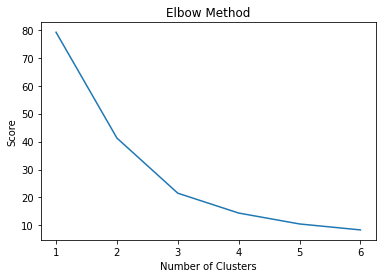
\includegraphics[scale=0.75]{figs/elbowgraph.png}
    \caption{Método de Elbow}
    \label{fig:melbow}
 \end{figure}

Por fim, o \emph{k-means} é aplicado a base de dados através do objeto $sklearn.cluster.KMeans$.
O parâmetro $n\_clusters$ recebe o número de clusters encontrado no passo anterior. 
O parâmetro $init$ indica a utilização do \emph{k-means++} na inicialização dos pontos centrais.
Já o parâmetro  $max\_inter$, define como 50 o número máximo de iterações do algoritmo \emph{k-means}.

\begin{lstlisting}[language=Python, caption=Vetorização dos dados]
kmeans = KMeans(n_clusters=n_clusters, init='k-means++', max_iter=50)
fit_data = kmeans.fit(Y)
pred_class = kmeans.predict(Y)

display(fit_data.labels_)
df['Cluster'] = fit_data.labels_
\end{lstlisting}

 \begin{figure}[H]
   \centering
   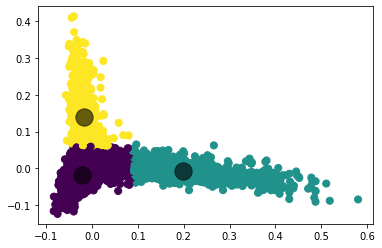
\includegraphics[scale=0.85]{figs/clustercloud.png}
    \caption{Distribuição dos clusters (dados vetorizados)}
    \label{fig:clustercloud}
 \end{figure}

\section{Resultados}
\subsection{Taxa de compressão}
Para validar a hipótese inicial, os dados particionados (aleatoriamente ou via compressão) foram comprimidos utilizando os algoritmos citados anteriormente.
Cada partição foi processada de maneira \textbf{individual}, portanto, a performance geral de cada algoritmo foi obtida a partir da média aritmética entre os resultados das $n$ partições.

Para compressão de dados sem perda o objetivo é reduzir o tamanho da mensagem, sem haver perda de informações.
Assim, uma das principais métricas de sucesso nestes algoritmos é a \textbf{taxa de compressão}.
Definimos a \textbf{taxa de compressão} como uma comparação entre o tamanho do documento codificado e o original.

\begin{equation}\label{eq:tf}
taxa~de~compressão = \frac{tamanho~do~documento~codificado}{tamanho~do~documento~original}
\end{equation}\label{eq:tf}

Definimos $\Delta$ como a métrica impacto da clusterização na taxa de compressão, que é obtida pela diferença entre os resultados com e sem a clusterização.
 \begin{figure}[H]
   \centering
   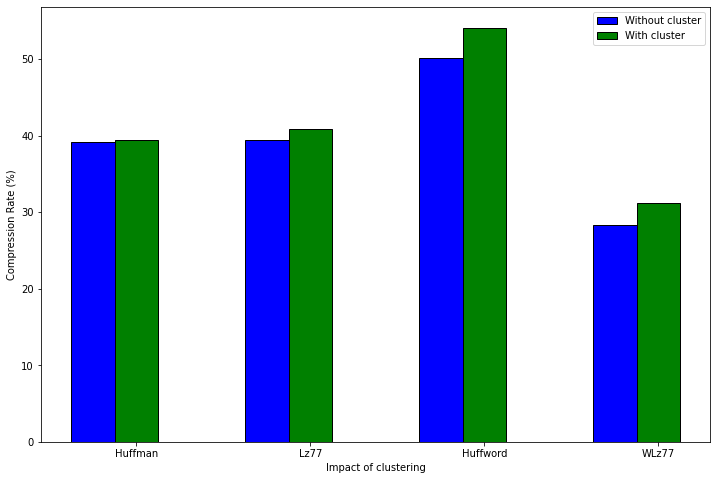
\includegraphics[scale=0.60]{figs/graphfinal.png}
    \caption{Impacto da clusterização na taxa de compressão}
    \label{fig:clusterfinalgraph}
 \end{figure}
 
 \begin{table}[H]
   \centering
   \caption{Impacto da clusterização na taxa de compressão} \label{tab:resultcomp}
   \begin{tabular}{|l|c|c|c|c|c|c|r|}
        \hline
        \small{Algoritmo} & \small{\% compressão} &  \small{\% compressão (clusters)} & \small{$\Delta$} \\ \hline
              Huffman   &   39.214536 & 39.395034 & 0.180498 \\ \hline
              Huffword  &   50.133603 & 54.096327 & 3.962724 \\ \hline
              LZ77        &   39.470517 & 40.795727 & 1.325210 \\ \hline
              WLZ77    &   28.369986 & 31.173907 & 2.803921 \\ \hline
  \end{tabular}
\end{table}

Conforme previsto no capítulo~\ref{cap:comp}, a tabela~\ref{tab:resultcomp} mostra que a clusterização teve um maior impacto nos algoritmos baseados em \textbf{palavras}.
Em especial, o maior $\Delta$ foi alcançado para o \emph{Huffword}, onde foi \textbf{alcançado uma melhoria de quase 4\%}. Curiosamente, a versão baseada em palavras do LZ77 se mostrou menos efetiva no geral do que sua versão canônica.

\subsection{Tempo de execução}
Outra métrica que auxilia na comparação entre os algoritmos é o \textbf{tempo de execução}.
Para isso, foi utilizada o comando \emph{\%time\%} do \emph{jupyter notebook} (que mede o tempo de execução da célula em que o comando foi inserido).

\begin{table}[H]
   \centering
   \caption{Tempo de execução dos algoritmos de compressão} \label{tab:vcode}
   \begin{tabular}{|l|c|c|c|c|c|c|r|}
        \hline
        \small{Algoritmo} & \small{Tempo de execução} & \small{Partição} \\ \hline
              Huffman   &   2.18s                        & aleatória \\ \hline
              Huffword  &   2.8s                          & aleatória \\ \hline
              LZ77        &   8min 24s                  & aleatória \\ \hline
              WLZ77    &   1h 37min 41s           & aleatória \\ \hline
              Huffman  &   3.08s                       & k-means \\ \hline
              Huffword &   3.66s                       & k-means \\ \hline
              LZ77       &   12min 24s               & k-means \\ \hline
              WLZ77   &   2h 30min 9s            & k-means \\ \hline
  \end{tabular}
\end{table}

Fica claro que as versões baseadas em palavra e clusterizadas via \emph{k-means}, consomem mais tempo de execução.
Este dado já era esperado, já que o aumento de símbolos semelhantes leva a mais \emph{tokenizações}, e por consequência maior tempo de processamento.

\section{Conclusão}
Neste trabalho, combinamos o uso da compressão \textbf{baseada} em palavras com a clusterização.
Os resultados experimentais confirmam as hipóteses levantadas previamente, 
e chega-se a conclusão de que a clusterização impacta \texbf{positivamente} a \textbf{taxa de compressão} de textos.
Entretanto, os experimentos também mostram um aumento nos recursos consumidos (tanto pelo pré-processamento, quanto pela compressão em si).
Os resultados apresentados neste trabalho podem ser úteis na implementação de ferramentas de compressão otimizadas, principalmente para grande bases de dados textuais.
\section{Trabalhos relacionados e melhorias}






%\chapter{Estado da Arte}\label{cap:estArte}

\lipsum[34]

\section*{Trabalhos Relacionados a Isto}\label{sec:primTrab}
\addcontentsline{toc}{section}{Trabalhos Relacionados a Isto}

\lipsum[34-36]
%\chapter{Materiais e Métodos}\label{cap:ferramentas}

\lipsum[43-45]

\section{Considerações Finais}

\lipsum[23]


% PARTE
%\part{Proposta}
%\chapter{Sistema Proposto}\label{cap:proposta}

Esse trabalho propõe um sistema de... 


\section{Primeira Parte do Sistema Proposto}

\lipsum[67]

\section{Considerações Finais}

\lipsum[68]


% PARTE
%\part{Parte Final}
%\chapter{Resultados e Discussão}\label{cap:resultados}

\lipsum[73]

\section{Base de Dados}

\lipsum[72]

\section{Considerações Finais}

\lipsum[74]
%\chapter*{Conclusões e Trabalhos Futuros}\label{cap:conclusao}
\addcontentsline{toc}{chapter}{Conclusão e Trabalhos Futuros}

\lipsum[81]

\section*{Conclusões}

\lipsum[82-84]

\section*{Trabalhos Futuros}

\lipsum[85] 

% ----------------------------------------------------------
% ELEMENTOS PÓS-TEXTUAIS (Referências, Glossário, Apêndices)
% ----------------------------------------------------------
\postextual

\begin{thebibliography}{9999}  
\bibitem[HL]{D.S Hirschberg}HIRSCHBERG, D.S; LELEWER D.A;
\emph{Data compression, }Computing Surveys 19.3, 1987.

\bibitem[Ble]{Guy E. Blelloch}BLELLOCH G.E;
\emph{Introduction to Data Compression, } Carnegie Mellon, 2013

\bibitem[BT]{Dimitri P. Bertsekas} BERTSEKAS D.P; TSITSIKLIS J.N;
\emph{Introduction to Probability} M.I.T, Lecture Notes Course 6.041-6.431, 2000

\end{thebibliography}
	
% Glossário (Consulte o manual)
%\glossary

% Apêndices
% % ----------------------------------------------------------
% Apêndices
% ----------------------------------------------------------

% ---
% Inicia os apêndices
% ---
\begin{apendicesenv}

% Imprime uma página indicando o início dos apêndices
\partapendices

% ----------------------------------------------------------
\chapter{Primeiro Apêncice}
% ----------------------------------------------------------

\lipsum[50] % Texto qualquer. REMOVER!!

% ----------------------------------------------------------
\chapter{Segundo apêndice com título tão grande quanto se queira porque ele já faz a quebra de linha da coisa toda}
% ----------------------------------------------------------
\lipsum[51-53] % Texto qualquer. REMOVER!!

\end{apendicesenv}
% ---

% Anexos
% % ----------------------------------------------------------
% Apêndices
% ----------------------------------------------------------

% ---
% Inicia os anexos
% ---
\begin{anexosenv}

% Imprime uma página indicando o início dos anexos
\partanexos

% ---
\chapter{Nome do Primeiro Anexo}
% ---
\lipsum[30] % Texto qualquer. REMOVER!!

% ---
\chapter{Nome de Outro Anexo}
% ---

\lipsum[32] % Texto qualquer. REMOVER!!

\end{anexosenv}

% Índice remissivo (Consultar manual)
%\phantompart
%\printindex

\end{document}
